%%%%%%%%%%%%%%%%%%%%%%%%%%%%%%%%%%%%%%%%%%%%%%%%%%%
%% P3: Phenomenology of Particle Physics                         
%%
%% Author:  André Rubbia                   		 
%%
%% Figure 17.20 Double differential cross-section divided by the factor $f$ (see text) as a function
%% of Bjorken $x$ in $ep$ scattering for data with $Q^2>1$~GeV$^2$.
%%
%% This work is licensed under the Creative Commons Attribution 4.0 International License. 
%% To view a copy of this license, visit http://creativecommons.org/licenses/by/4.0/ or 
%% send a letter to Creative Commons, PO Box 1866, Mountain View, CA 94042, USA.
%%
%%%%%%%%%%%%%%%%%%%%%%%%%%%%%%%%%%%%%%%%%%%%%%%%%%%

\documentclass[a4paper,10pt]{article}

\usepackage[T1]{fontenc}
\usepackage[utf8]{inputenc}
\usepackage{lmodern}
\usepackage[labelfont=bf]{caption}
\usepackage{upgreek}

\usepackage{tikz}
\usepackage{pgfplots}
\pgfplotsset{compat=1.17}
\usepgfplotslibrary{ternary}
\usepgfplotslibrary{fillbetween}
\usepgfplotslibrary{external}

\def\d{\mathrm{d}}

\begin{document}

%%%%%%%%%%%%%%%   FIGURE  %%%%%%%%%%%%%%%%%%%%%%%%%%%%%%
\begin{figure}[htb]
\begin{center}
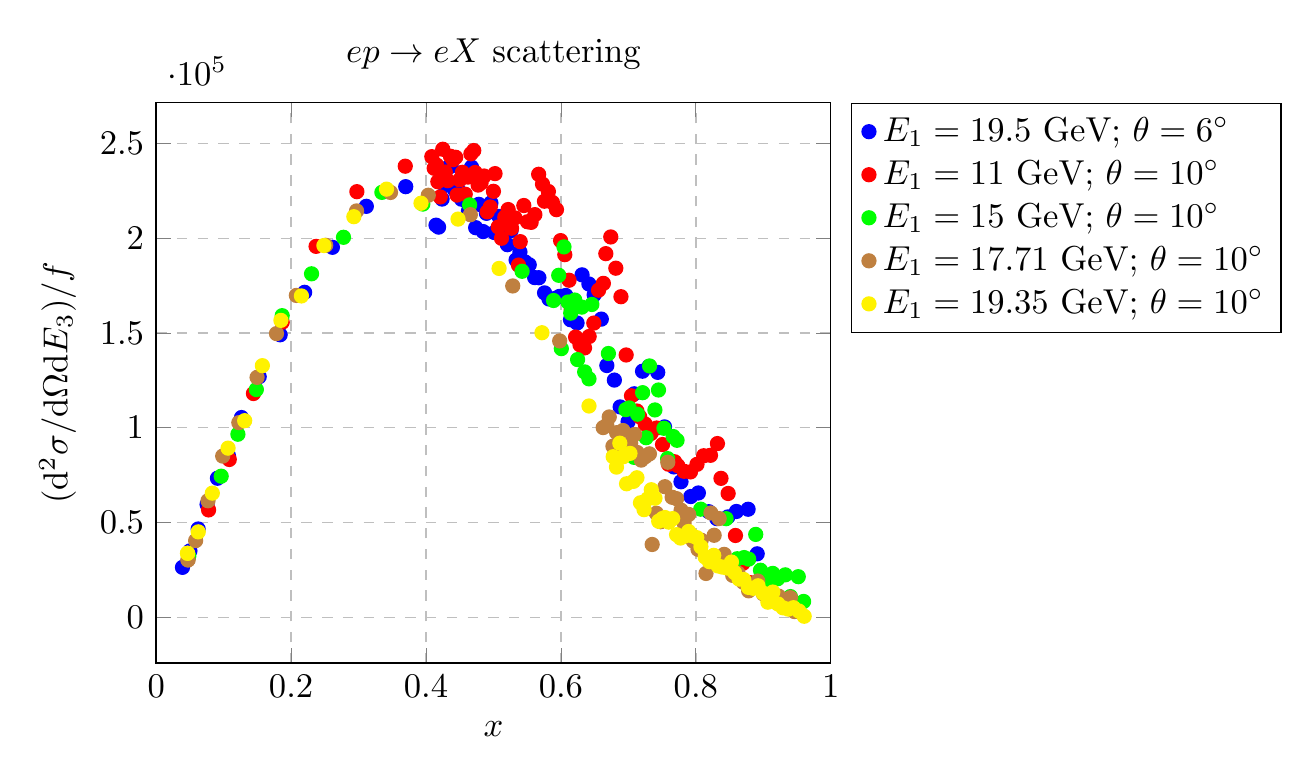
\begin{tikzpicture}[scale=1.25]
\begin{axis}[
    title={$ep\rightarrow eX$ scattering},
    xlabel={$x$},
    ylabel={$({\d^2\sigma}/{\d\Omega\d E_3})/f$},
    xmin=0, xmax=1,
	legend style={legend pos = outer north east},
	legend cell align = {left},
    	ymajorgrids=true,
    	xmajorgrids=true,
    grid style=dashed,
]

%%% ep->ex, E=19.5, theta=6deg
\addplot[
    color=blue,
    only marks,
    ]
    coordinates {
(0.909496,18614.3)(0.890974,33524.3)(0.877516,57030.6)(0.860123,55868.4)(0.847473,52981.7)(0.83111,52085.5)(0.819198,55747.6)(0.803775,65615.4)(0.792539,63733)(0.777978,71536.6)(0.76736,79350.7)(0.753591,100468)(0.743543,129226)(0.730502,132327)(0.720979,129836)(0.708611,117929)(0.699572,103218)(0.687825,110998)(0.679236,125159)(0.668065,132836)(0.659891,157317)(0.649255,170186)(0.641468,175862)(0.631329,180660)(0.623902,155274)(0.614226,156984)(0.607134,169797)(0.59789,169305)(0.591111,168221)(0.582271,167967)(0.575785,171149)(0.567323,179142)(0.561112,179215)(0.553003,185963)(0.547049,187421)(0.539273,192701)(0.533561,188538)(0.526097,204002)(0.520612,196585)(0.513442,206619)(0.508171,211450)(0.501278,202987)(0.496208,218575)(0.489577,213099)(0.484697,203480)(0.478312,217856)(0.473612,205549)(0.46746,237473)(0.46293,214350)(0.456999,233916)(0.45263,220570)(0.446908,225908)(0.442691,225366)(0.437167,237989)(0.433095,237414)(0.427759,227801)(0.423824,220627)(0.418666,205835)(0.414863,206866)(0.369936,227174)(0.311544,216807)(0.26124,195195)(0.220061,171445)(0.183802,149055)(0.152711,126961)(0.126455,105394)(0.107085,85333.8)(0.0907922,73380.1)(0.0754371,59577.3)(0.0622252,46612.9)(0.050008,35052.7)(0.0389541,26379.9)
};

%%% ep->ex, E=11, theta=10deg
\addplot[
    color=red,
    only marks,
    ]
    coordinates {
(0.881173,18283.4)(0.869843,28529.6)(0.858753,43199.1)(0.847896,65360.5)(0.837263,73333)(0.832029,91678.3)(0.821721,85479.4)(0.811621,85247.5)(0.801723,80710.8)(0.792021,76734)(0.78251,77058.5)(0.773183,80048.2)(0.768587,82069.2)(0.759527,80778.9)(0.750639,91153.4)(0.741918,99883)(0.733359,96968)(0.724958,101950)(0.71671,105854)(0.712643,108844)(0.704617,116884)(0.696735,138403)(0.688993,169136)(0.681386,184170)(0.673912,200661)(0.666567,191850)(0.662941,176163)(0.655783,172577)(0.648745,155222)(0.641826,148148)(0.635021,142127)(0.628328,143730)(0.621744,147844)(0.615267,162495)(0.612068,177824)(0.605746,191313)(0.599525,198725)(0.593401,215049)(0.587373,218862)(0.581439,224626)(0.575596,219499)(0.572708,228519)(0.566998,233706)(0.561374,212426)(0.555835,208350)(0.550377,208673)(0.545001,217233)(0.539703,198182)(0.537083,185804)(0.5319,210714)(0.526792,205249)(0.521756,215111)(0.516792,211087)(0.511898,199959)(0.507073,205941)(0.502314,234060)(0.49996,224727)(0.495299,216481)(0.490702,213900)(0.486167,232791)(0.481694,229232)(0.47728,228009)(0.472925,234641)(0.470769,246238)(0.4665,244494)(0.462286,232222)(0.458127,223221)(0.454022,234747)(0.44997,230775)(0.445969,222757)(0.443988,242672)(0.440062,241388)(0.436186,243242)(0.432359,230346)(0.428578,234882)(0.424845,246916)(0.421157,221754)(0.417513,229775)(0.415708,238596)(0.412131,236874)(0.408596,243011)(0.36926,237973)(0.297511,224540)(0.237044,195693)(0.186787,155679)(0.144169,118062)(0.108355,83285.8)(0.0776836,56680.5)
      };

 %%%  ep->ex, E=15, theta=10deg
    \addplot[
    color=green,
    only marks,
    ]
    coordinates {
(0.959758,8404.96)(0.951872,21464.7)(0.940234,10968.5)(0.932601,22429.3)(0.921333,20391.1)(0.913941,23203.9)(0.903027,17792.5)(0.895865,24856.5)(0.888791,43760.6)(0.878345,30728.4)(0.871487,31543.5)(0.861355,30914.6)(0.854703,26991.8)(0.844873,52060.9)(0.807254,57068.6)(0.77215,93392.8)(0.766526,95388.5)(0.758206,83731.2)(0.752735,99742.6)(0.744641,119921)(0.739317,109410)(0.731437,132612)(0.726255,94766.1)(0.721127,118516)(0.713535,107156)(0.708541,84399.2)(0.701146,110488)(0.696279,109571)(0.670386,139164)(0.645882,165049)(0.641567,125803)(0.635173,129482)(0.630961,163640)(0.624719,135968)(0.620607,167369)(0.614511,160454)(0.610495,166330)(0.604541,195409)(0.600617,141744)(0.59673,180428)(0.589062,167135)(0.542441,182541)(0.464664,217580)(0.395267,218001)(0.334581,224165)(0.277653,200478)(0.230326,181218)(0.186794,159136)(0.148482,120165)(0.121109,96590.1)(0.0963642,74465.9)(0.0481236,32175.6)(0.0481236,32175.6)
};

 %%%  ep->ex, E=17.71, theta=10deg
    \addplot[
    color=brown,
    only marks,
    ]
    coordinates {
(0.94615,3072)(0.940193,10387.7)(0.931366,8926.2)(0.922664,11225.7)(0.914086,9041.12)(0.908435,11932.7)(0.900057,12359.9)(0.891795,19160.3)(0.883648,15696.9)(0.878279,13998.5)(0.870317,18523.5)(0.862463,23314.5)(0.854715,22143.9)(0.849607,28539.7)(0.842031,33230.5)(0.834555,52110.9)(0.827177,43296.8)(0.822313,55053.8)(0.815095,23168.4)(0.80797,40725.3)(0.803271,35880.7)(0.796298,40204.3)(0.789414,54285)(0.782617,49714.8)(0.778133,56521.8)(0.771477,62609.7)(0.764903,63353.6)(0.758411,81825.6)(0.754127,68926.9)(0.747767,50451.4)(0.741484,54922.4)(0.735277,38448.4)(0.73118,86251)(0.725096,84755.5)(0.719085,82962.5)(0.713144,86955.8)(0.709223,96479.7)(0.703398,91937.5)(0.697641,86819.4)(0.69195,98559.3)(0.688193,90851)(0.68261,97430.5)(0.677092,90261.9)(0.671635,105704)(0.668032,101325)(0.662678,100106)(0.598164,145812)(0.528557,174813)(0.465741,212397)(0.403367,222643)(0.347358,224117)(0.297059,214388)(0.251288,196255)(0.207797,169814)(0.178355,149683)(0.14958,126585)(0.122502,102715)(0.0985872,85074.6)(0.0767915,61507.2)(0.0584987,40483.3)(0.0471464,30319.2)(0.0471464,30319.2)
};

 %%%  ep->ex, E=19.35, theta=10deg
    \addplot[
    color=yellow,
    only marks,
    ]
    coordinates {
  (0.960613,597.121)(0.952634,3354.54)(0.944754,5104.25)(0.936972,4350.15)(0.929285,5030.79)(0.921692,7088.58)(0.914191,13358.5)(0.906781,8011.66)(0.89946,12875.1)(0.892227,16664.6)(0.885079,15347.5)(0.878015,15803.4)(0.871034,19959.5)(0.864134,20174.4)(0.857315,23666)(0.852812,29180.1)(0.846122,26059.1)(0.839509,26520.8)(0.832971,27112.9)(0.826506,32709.5)(0.820114,29390.4)(0.813794,31818.8)(0.807543,37265)(0.801361,42065.9)(0.795247,42949.9)(0.7892,45309.3)(0.783219,42875.7)(0.777302,41841.5)(0.771448,43619.7)(0.765657,52104.3)(0.759928,50233.9)(0.754259,52654.3)(0.750512,52123.2)(0.744942,50690.7)(0.73943,62856.2)(0.733975,67326.2)(0.728576,62480.6)(0.723233,56820.9)(0.717944,60426)(0.712708,73630.1)(0.707526,71737.8)(0.702396,86487.9)(0.697317,70470.7)(0.692288,84718)(0.68731,91872.3)(0.68238,79266.5)(0.677499,84752.1)(0.641608,111494)(0.571899,150137)(0.508321,184054)(0.447491,210073)(0.392572,218434)(0.341492,225872)(0.29303,211339)(0.248629,196120)(0.215309,169533)(0.184899,156651)(0.15743,132768)(0.131196,103746)(0.106565,89260.5)(0.0832183,65523.4)(0.0623306,45106)(0.0464986,33808.6)(0.0464986,33808.6)
};

     \legend{
      $E_1=19.5$~GeV; $\theta=6^\circ$,
      $E_1=11$~GeV; $\theta=10^\circ$,
      $E_1=15$~GeV; $\theta=10^\circ$,
      $E_1=17.71$~GeV; $\theta=10^\circ$,
      $E_1=19.35$~GeV; $\theta=10^\circ$
	}
\end{axis}
\end{tikzpicture}
\caption{Double differential cross-section divided by the factor $f$ (see text) as a function
of Bjorken $x$ in $ep$ scattering for data with $Q^2>1$~GeV$^2$.
Compare with Figures 16.9 and 16.10 of the book.
Adapted with permission from
E.~D. Bloom {\em et~al.}, ``High-energy inelastic $e\ensuremath{-}p$ scattering
  at 6 and 10 deg,'' {\em Phys. Rev. Lett.}, vol.~23, pp.~930--934, Oct 1969.}
\end{center}
\end{figure}
%%%%%%%%%%%%%%%  END FIGURE  %%%%%%%%%%%%%%%%%%%%%%%%%%%%%%
%

\end{document}
